\subsectionaddtolist{الف}

{
	\centering{
		
		 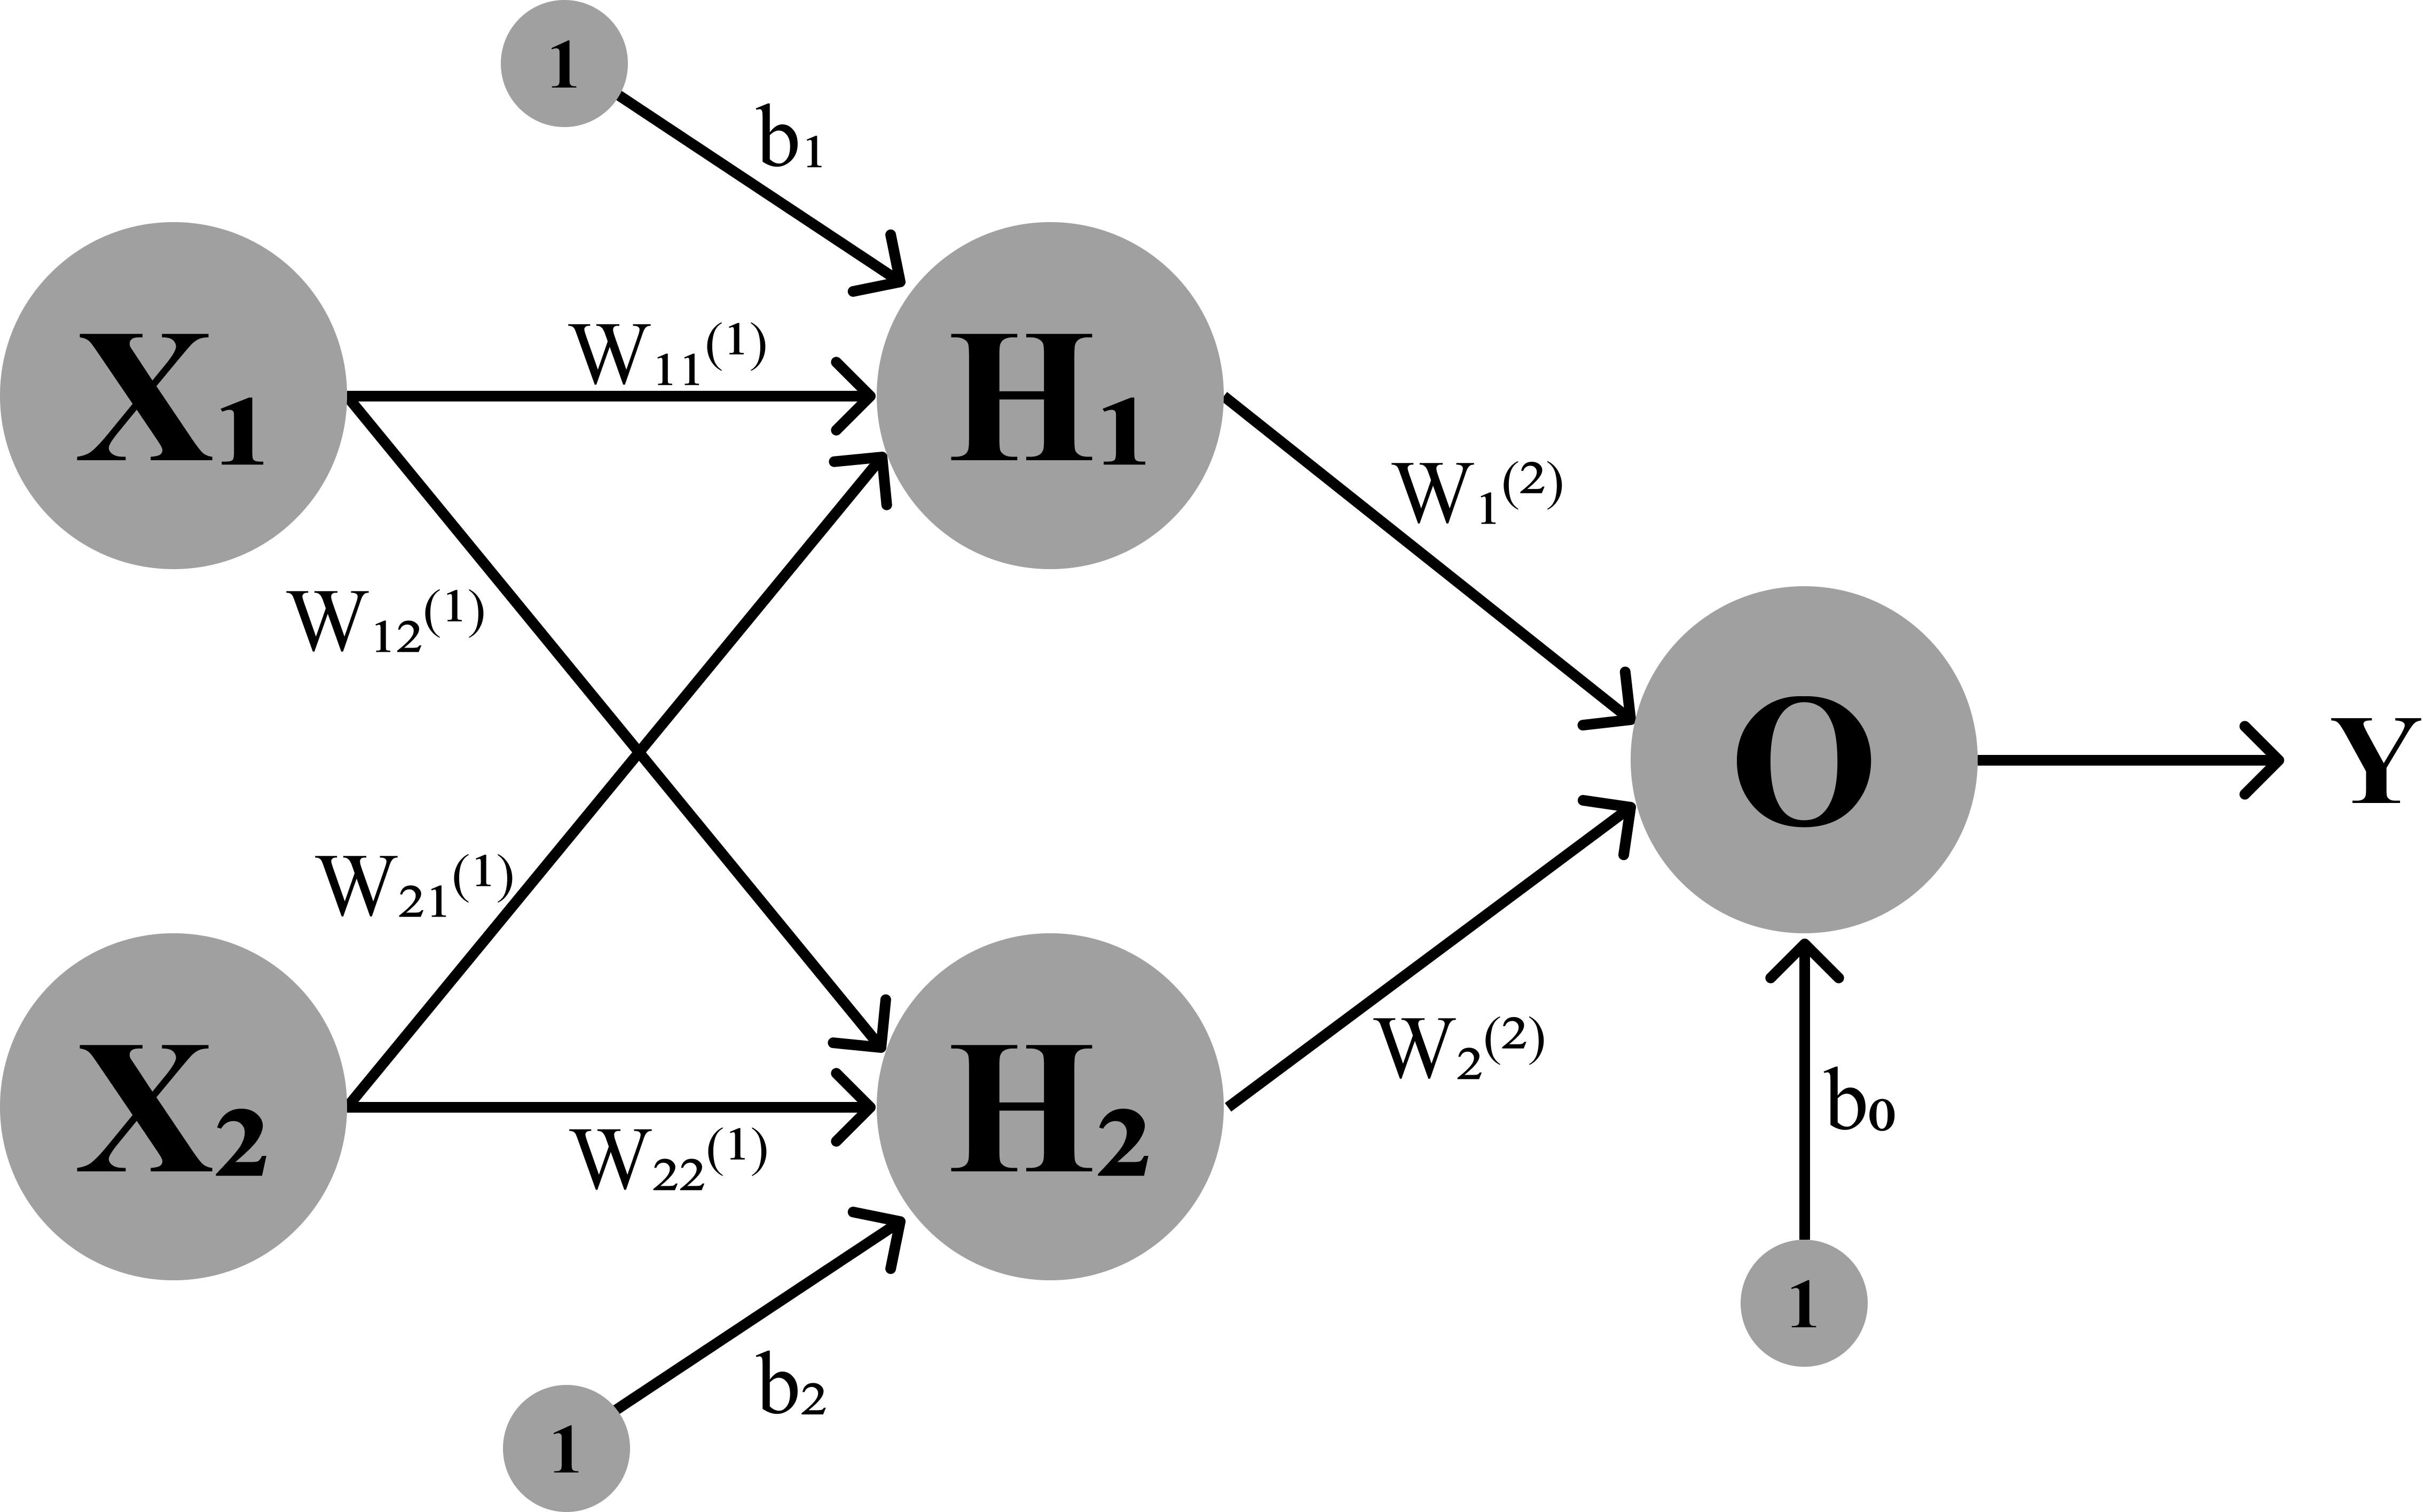
\includegraphics[width=0.4\textwidth]{figs/3.png}
		
	}
}

این شبکه دارای 6 وزن و 3 بایاس هست، پس جمعا دارای ۹ پارامتر قابل یادگیری هستیم.


\subsectionaddtolist{ب}


تابع ReLU به صورت زیر تعریف می‌شود:
\[
\text{ReLU}(x) = \max(0, x)
\]

{
	\centering{
		
		 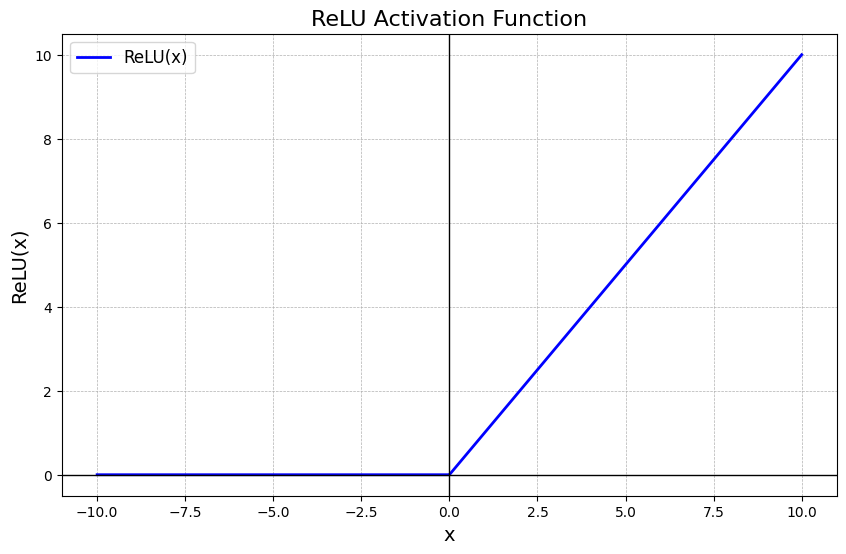
\includegraphics[width=0.4\textwidth]{figs/4.png}
		
	}
}


\begin{table}
	\centering
	\begin{tabular}{|c|c|c|}
		\hline
		\textbf{ویژگی} & \textbf{ReLU} & \textbf{سیگموید} \\
		\hline
		محدوده خروجی & $[0, +\infty)$ & $(0, 1)$ \\
		\hline
		تابع مشتق‌پذیر & خیر (در $x=0$ ناپیوستگی دارد) & بله \\
		\hline
		مسأله ناپدید شدن گرادیان & ندارد یا بسیار کمتر & دارد \\
		\hline
		رفتار در نواحی منفی & خروجی صفر (امکان خاموشی نورون) & خروجی نزدیک به صفر \\
		\hline
	\end{tabular}
\end{table}

همچنین اگر وزن‌ها طوری تنظیم شوند که ورودی نورون همیشه منفی باشد، ReLU همیشه صفر می‌شود و نورون دیگر هیچ‌وقت فعال نمی‌شود.

{خروجی تابع ReLU برای ورودی $-2$:}
\[
\text{ReLU}(-2) = \max(0, -2) = 0
\]

\subsectionaddtolist{پ}



برای نورون اول:
\[
z_1^{(1)} = w_{11}^{(1)} x_1 + w_{12}^{(1)} x_2 + b_1^{(1)} = 1 \times 1 + (-1) \times 1 + 0 = 0
\]
\[
a_1^{(1)} = \text{ReLU}(z_1^{(1)}) = \max(0, 0) = 0
\]

برای نورون دوم:
\[
z_2^{(1)} = w_{21}^{(1)} x_1 + w_{22}^{(1)} x_2 + b_2^{(1)} = 2 \times 1 + 1 \times 1 + 1 = 4
\]
\[
a_2^{(1)} = \text{ReLU}(z_2^{(1)}) = \max(0, 4) = 4
\]

{لایه خروجی:}

\[
y_{\text{pred}} = w_1^{(2)} a_1^{(1)} + w_2^{(2)} a_2^{(1)} + b^{(2)} = 2 \times 0 + (-1) \times 4 + 0 = -4
\]

مقدار واقعی:
\[
y = 5
\]

تابع خطای میانگین مربعات:
\[
\text{MSE} = \frac{1}{2}(y_{\text{pred}} - y)^2 = \frac{1}{2}(-4 - 5)^2 = \frac{1}{2}(81) = {40.5}
\]


\subsectionaddtolist{ت}

با استفاده از این فرمول‌ها، وزن‌ها را آپدیت می‌کنیم:

\[
\Delta w_{ij} = \eta \, \delta_j \, o_i
\]

\[
\delta_j =  f'(z_j) \cdot (t_j - o_j) \quad \text{output }
\]

\[
\delta_j =  f'(z_j) \cdot \sum_k \delta_k \, w_{kj} \quad \text{hidden }
\]


\subsubsection*{محاسبه \lr{$\delta$} برای نورون‌های خروجی}

با توجه به استفاده از تابع هویت (مشتق برابر ۱):

\[
\delta = t - o = 5 - (-4) = 9
\]



برای نورون اول در لایه پنهان:

\[
\Delta w_1^{(2)} = 0.1 \cdot 9 \cdot 0 = 0
\longrightarrow w_1^{(2)} = 2 + 0 = 2
\]

برای نورون دوم در لایه پنهان:

\[
\Delta w_2^{(2)} = 0.1 \cdot 9 \cdot 4 = 3.6
\longrightarrow w_2^{(2)} = -1 + 3.6 = 2.6
\]


برای بایاس:

\[
\Delta b^{(2)} = 0.1 \cdot 9 = 0.9
\longrightarrow b^{(2)} = 0 + 0.9 = 0.9
\]


\subsubsection*{محاسبه \lr{$\delta$} برای نورون‌های پنهان}

مقادیر ورودی نورون‌های پنهان:
\[
z_1^{(1)} = 0 \longrightarrow f'(z_1) = 0
\quad , \quad
z_2^{(1)} = 4 \longrightarrow f'(z_2) = 1
\]


برای نورون اول:
\[
\delta_1^{(1)} = 0 \times 9 \times 2 = 0
\]

برای نورون دوم:
\[
\delta_2^{(1)} = 1 \times 9 \times (-1) = -9
\]


نورون اول:
\[
\delta_1 = 0 \longrightarrow \Delta w_{11} = \Delta w_{12} = 0 \longrightarrow \text{بدون تغییر}
\]

نورون دوم:
\[
\Delta w_{21} = 0.1 \times (-9) \times 1 = -0.9  \longrightarrow w_{21} = 2 - 0.9 = 1.1
\]
\[
\Delta w_{22} = 0.1 \times (-9) \times 1 = -0.9  \longrightarrow w_{22} = 1 - 0.9 = 0.1
\]
\[
\Delta b_2 = 0.1 \times (-9) = -0.9  \longrightarrow b_2 = 1 - 0.9 = 0.1
\]



نرخ یادگیری نقش تعیین‌کننده‌ای در به‌روزرسانی وزن‌ها دارد:
\begin{itemize}
	\item اگر نرخ یادگیری بیش از حد کوچک باشد، آموزش بسیار کند پیش می‌رود و شبکه ممکن است در مینیمم محلی گیر کند.
	\item اگر نرخ یادگیری بیش از حد بزرگ باشد، به‌روزرسانی وزن‌ها بسیار شدید می‌شود و ممکن است باعث نوسان یا واگرایی در روند یادگیری شود.
\end{itemize}

بنابراین، انتخاب مقدار مناسب برای $\eta$ بسیار حیاتی است و معمولاً به کمک تجربه یا تنظیمات خودکار (مانند کاهش تطبیقی نرخ یادگیری) انجام می‌شود.


\subsectionaddtolist{ث}


\subsubsection*{الگوریتم \lr{Gradient Descent} کلاسیک}

\begin{itemize}
	\item در این الگوریتم، پارامترها با استفاده از گرادیان کلی تابع هزینه نسبت به پارامترها، به‌روزرسانی می‌شوند:
	\[
	\theta \leftarrow \theta - \eta \cdot \nabla_\theta J(\theta)
	\]
	\item نیاز به انتخاب یک نرخ یادگیری ثابت دارد.
	\item ممکن است در دره‌های باریک یا سطوح پرنوسان کند پیش برود یا گیر کند.
\end{itemize}

\subsubsection*{الگوریتم \lr{Adam (Adaptive Moment Estimation)}}

\begin{itemize}
	\item Adam از دو مفهوم استفاده می‌کند:
	\begin{enumerate}
		\item \textbf{میانگین گرادیان‌ها (momentum)} – مانند سرعت حرکت.
		\item \textbf{میانگین مربعات گرادیان‌ها (RMS)} – کنترل نوسان.
	\end{enumerate}
	\item فرمول‌های اصلی:
	\[
	m_t = \beta_1 m_{t-1} + (1 - \beta_1) \nabla_\theta J(\theta)
	\]
	\[
	v_t = \beta_2 v_{t-1} + (1 - \beta_2) (\nabla_\theta J(\theta))^2
	\]
	\[
	\hat{m}_t = \frac{m_t}{1 - \beta_1^t}, \quad \hat{v}_t = \frac{v_t}{1 - \beta_2^t}
	\]
	\[
	\theta \leftarrow \theta - \eta \cdot \frac{\hat{m}_t}{\sqrt{\hat{v}_t} + \varepsilon}
	\]
\end{itemize}

\subsubsection*{تفاوت‌های کلیدی بین \lr{Gradient Descent} و \lr{Adam}}

\begin{itemize}
	\item \textbf{نرخ یادگیری:}  
	در \lr{Gradient Descent} نرخ یادگیری یک مقدار ثابت است و نیاز به تنظیم دقیق دارد، در حالی‌که \lr{Adam} نرخ یادگیری را به صورت تطبیقی برای هر پارامتر تنظیم می‌کند.
	
	\item \textbf{سرعت همگرایی:}  
	\lr{Gradient Descent} معمولاً کندتر همگرا می‌شود، به‌خصوص در فضاهای با توپوگرافی پیچیده؛ در مقابل، \lr{Adam} با استفاده از مومنتوم و میانگین مربعات گرادیان، سریع‌تر به جواب می‌رسد.
	
	\item \textbf{حساسیت به مقیاس داده‌ها:}  
	\lr{Gradient Descent} نسبت به مقیاس داده‌ها حساس است و اغلب نیاز به نرمال‌سازی دارد، در حالی که \lr{Adam} این مسئله را با نرمال‌سازی درونی کاهش می‌دهد.
	
	\item \textbf{نیاز به تنظیمات دستی:}  
	در \lr{Gradient Descent} انتخاب نرخ یادگیری حیاتی است و به تنظیم دقیق نیاز دارد؛ ولی \lr{Adam} اغلب با مقادیر پیش‌فرض (مثل $\beta_1 = 0.9$ و $\beta_2 = 0.999$) به خوبی کار می‌کند.
	
	\item \textbf{مصرف حافظه:}  
	\lr{Gradient Descent} حافظه بسیار کمی مصرف می‌کند؛ اما \lr{Adam} برای هر پارامتر دو متغیر (میانگین و واریانس گرادیان) ذخیره می‌کند و نیاز به حافظه بیشتری دارد.
\end{itemize}


\subsubsection*{مزایا و شرایط مناسب استفاده از \lr{Adam}}

\begin{itemize}
	\item مناسب برای مسائل با داده‌های بزرگ، ویژگی‌های زیاد یا نویز بالا.
	\item عملکرد خوب بدون نیاز به تنظیم زیاد هایپرپارامترها.
	\item مناسب برای شبکه‌های عمیق مانند CNN و RNN .
\end{itemize}

\subsubsection*{ضعف بالقوه Adam}

\begin{itemize}
	\item گاهی در نزدیکی مینیمم بهینه عمومی (Global-Minima) نمی‌رسد.
	\item به‌روزرسانی‌ها ممکن است ناپایدار شوند در صورتی که داده‌ها کاملاً نرمال‌سازی نشده باشند.
	\item در برخی مسائل ساده، GD یا SGD بهتر عمل می‌کنند.
\end{itemize}

\subsectionaddtolist{ج}



\subsubsection*{۱. استفاده از داده‌افزایی (Data-Augmentation)}
در مسائل بینایی ماشین، با چرخش، کشیدن، برش، نویزگذاری یا فلیپ کردن تصاویر می‌توان حجم داده‌ها را افزایش داد و مدل را از یادگیری جزئیات خاص داده‌ها بازداشت.

\subsubsection*{۲. تنظیم وزن‌ها (Weight-Regularization)}
با استفاده از جریمه‌هایی مانند $L_1$ و $L_2$ روی وزن‌ها، از بزرگ شدن بیش از حد وزن‌ها جلوگیری شده و مدل ساده‌تری ساخته می‌شود:
\[
\text{Loss} = \text{MSE} + \lambda \sum_i w_i^2
\]

\subsubsection*{۳. توقف زودهنگام (Early-Stopping)}
مدل در هنگام آموزش به محض افزایش خطای اعتبارسنجی (Validation) متوقف می‌شود، تا از بیش‌برازش جلوگیری شود.

\subsubsection*{۴. کاهش پیچیدگی مدل}
با کاهش تعداد لایه‌ها یا تعداد نورون‌ها در هر لایه، ظرفیت مدل کاهش می‌یابد و از یادگیری نویز جلوگیری می‌شود.

\subsubsection*{آیا افزایش تعداد نورون‌های پنهان همیشه مفید است؟}
خیر. افزایش بیش از حد نورون‌ها در لایه‌های پنهان باعث افزایش ظرفیت مدل و خطر بیش‌برازش می‌شود. در حالی که ممکن است دقت روی داده‌های آموزشی بالا برود، عملکرد مدل روی داده‌های جدید (تست) کاهش می‌یابد.

\subsubsection*{مکانیزم Dropout}

\textbf{تعریف:}
Dropout تکنیکی است که در هر مرحله از آموزش، به‌طور تصادفی برخی نورون‌ها (و وزن‌های متصل به آن‌ها) غیرفعال می‌شوند.

\paragraph{مزایا:}
\begin{itemize}
	\item جلوگیری از وابستگی بیش از حد به نورون‌های خاص
	\item نوعی ensemble ساده‌سازی‌شده از مدل‌های مختلف ایجاد می‌کند
	\item بهبود تعمیم‌پذیری (generalization)
\end{itemize}

\paragraph{محدودیت‌ها:}
\begin{itemize}
	\item ممکن است سرعت همگرایی را کاهش دهد
	\item نیاز به تنظیم دقیق نرخ dropout دارد
	\item گاهی در شبکه‌های بازگشتی (RNN) باعث بی‌ثباتی در حافظه زمانی می‌شود
\end{itemize}

\subsectionaddtolist{چ}

اگر مدل روی داده‌های آموزش عملکرد خوبی دارد اما روی داده‌های آزمایش (تست) نتایج ضعیفی ارائه می‌دهد، این نشانه‌ای از {بیش‌برازش (Overfitting)} است. در این حالت، مدل به‌جای یادگیری الگوهای کلی، جزئیات خاص و نویزهای داده‌های آموزش را یاد گرفته و قابلیت تعمیم‌دهی به داده‌های جدید را از دست داده است.

\subsubsection*{مفهوم \lr{Early Stopping}}


{Early-Stopping} تکنیکی برای جلوگیری از بیش‌برازش است که در آن فرآیند آموزش مدل در صورت افزایش خطای اعتبارسنجی (validation-error) متوقف می‌شود. ایده اصلی آن است که مدل را در نقطه‌ای متوقف کنیم که بهترین عملکرد را روی داده‌های اعتبارسنجی داشته باشد، نه الزاماً در پایان تمامی epoch ها .

\begin{itemize}
	\item در هر epoch ، مدل روی مجموعه اعتبارسنجی ارزیابی می‌شود.
	\item اگر بهبود معناداری در خطای اعتبارسنجی طی چند دوره مشاهده نشود، آموزش متوقف می‌شود.
	\item وزن‌هایی که در بهترین عملکرد ثبت شده‌اند، به‌عنوان مدل نهایی در نظر گرفته می‌شوند.
\end{itemize}

\subsubsection*{انتخاب تابع خطا در داده‌های دارای نویز}

در حضور نویز یا داده‌های پرت (outliers) ، استفاده از تابع خطای \lr{MSE} توصیه نمی‌شود، چرا که:
\begin{itemize}
	\item \lr{MSE} مجذور خطا را در نظر می‌گیرد و به خطاهای بزرگ وزن بیشتری می‌دهد.
	\item داده‌های پرت تأثیر زیادی بر به‌روزرسانی وزن‌ها دارند.
\end{itemize}

\textbf{پیشنهاد:} استفاده از توابع مقاوم‌تر مانند:
\begin{itemize}
	\item \lr{MAE (Mean Absolute Error)}: به خطاهای بزرگ حساس نیست و در برابر نویز مقاوم‌تر است.
	\item \lr{Huber Loss}: ترکیبی از MSE و MAE است؛ برای خطاهای کوچک مانند MSE عمل می‌کند و برای خطاهای بزرگ مانند MAE.
\end{itemize}
